% torsion angles
The backbone of a polypeptide chain is flexible and changes shape by rotating around its bonds.
There are three different angles of rotation for every residue in a protein,
also called torsion angles (Fig. \ref{fig:torsion_angles}).
The rotation angle around the peptide bond, 
connecting the amino group with carboxylic acid group,
is called $\omega$.
The torsion angles around the bond that connect the amino group with $\alpha$-carbon is $\phi$,
and $\psi$ is the angle around the bond that connects the $\alpha$-carbon with the carboxylic acid group.

A protein in disordered state is highly dynamical and can rotate relatively freely around its torsion angles.
In folding the proteins fixes most of these torsion angles, 
thereby losing entropy.
For folding to be spontaneous, 
the protein needs to compensate for this loss of entropy with a negative change in enthalpy.
This is done by forming molecular interactions 
(e.g. hydrogen bonds, Van Der Waals interactions, electrostatic interactions, etc).
Should all the torsion angles be able to rotate the full 360 degrees,
the entropic loss would be to great to overcome
and the protein would never fold.
This is only a simplified explanation,
the reality is more complex as also the entropy and enthalpy of the surrounding environment,
especially the water molecules, have to be taken in to account.

Torsion angles are restricted however.
The $\omega$ angle describes the rotation around the peptide bond.
Because peptide bonds have a partial double-bond character, 
only two conformations are energetically allowed: 
cis conformation (0 degrees) (Fig. \ref{fig:cis}),
and trans conformation (180 degrees) (Fig. \ref{fig:trans}).
For sterical reasons,
the trans conformation is more frequently observed.
For similar sterical reasons,
not all $\phi$ and $\psi$ angle combinations are  physically possible.
Allowed combination can be visualised on a Ramachandran plot
(\cite{berg2015}).
Within these allowed Ramachandran plot regions,
regular repeating arrangements can arise to form secondary structures,
The most common being $\alpha$-helices and $\beta$-strands.

~\begin{figure}[h!]
	~\begin{subfigure}[b]{0.32\linewidth}
		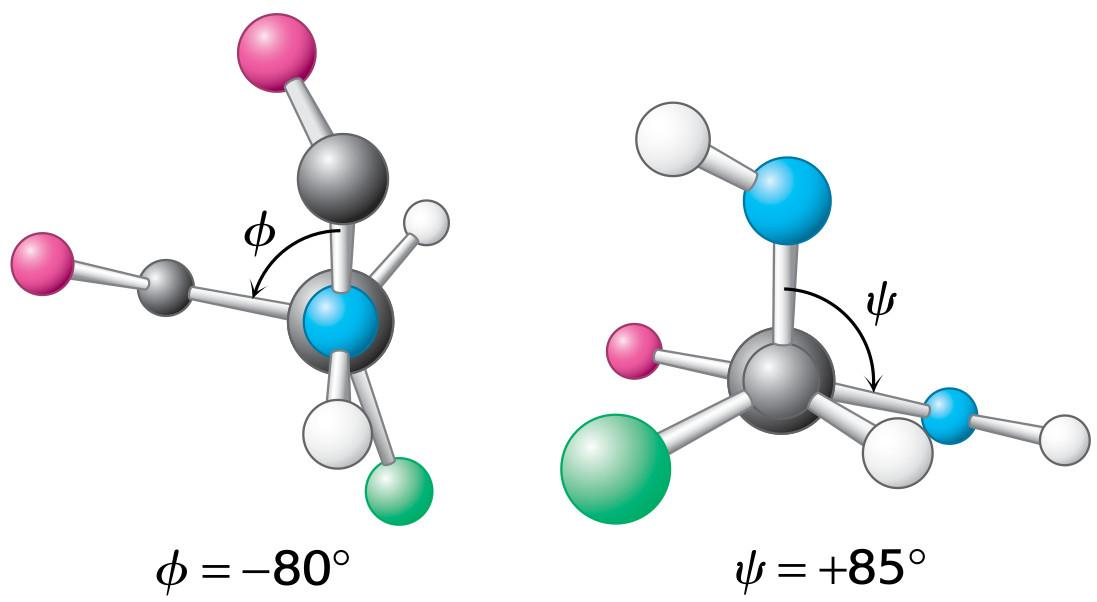
\includegraphics[width=\linewidth]{./literature_review/proteins/secundary_structure/img/torsion_angles.jpg}
		\caption{\textbf{Torsion angles}}
		\label{fig:torsion_angles}
	~\end{subfigure}
	~\begin{subfigure}[b]{0.32\linewidth}
		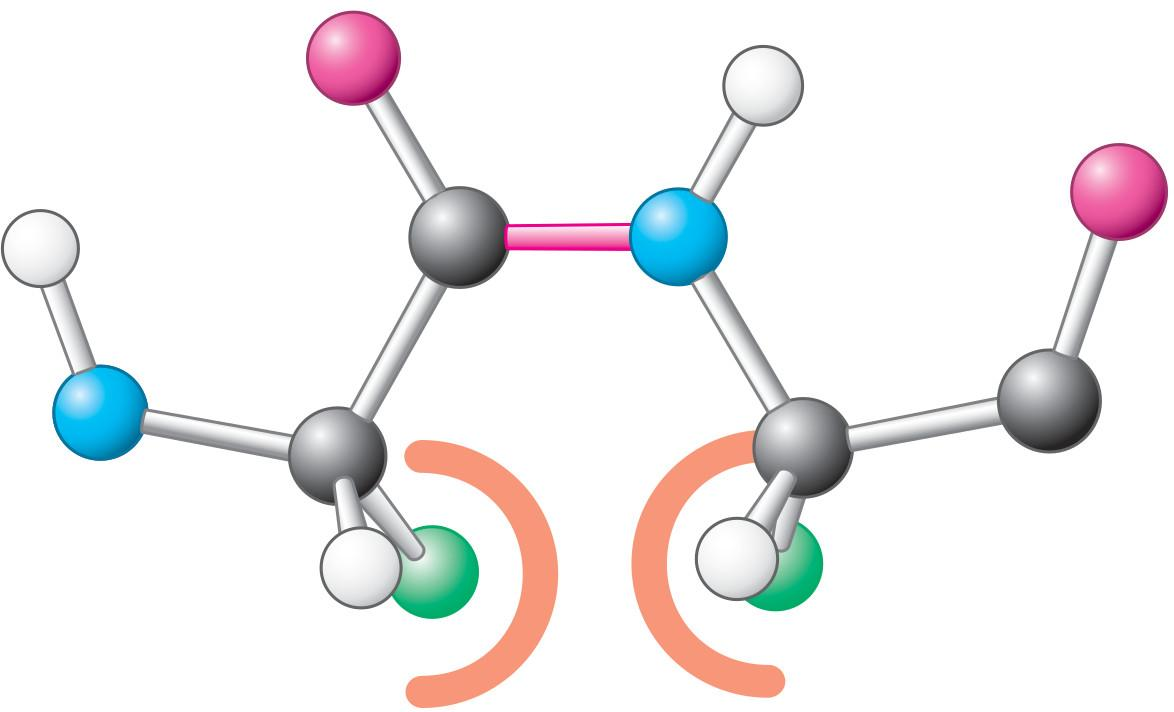
\includegraphics[width=\linewidth]{./literature_review/proteins/secundary_structure/img/cis.jpg}
		\caption{\textbf{Cis}}
		\label{fig:cis}
	~\end{subfigure}
	~\begin{subfigure}[b]{0.32\linewidth}
		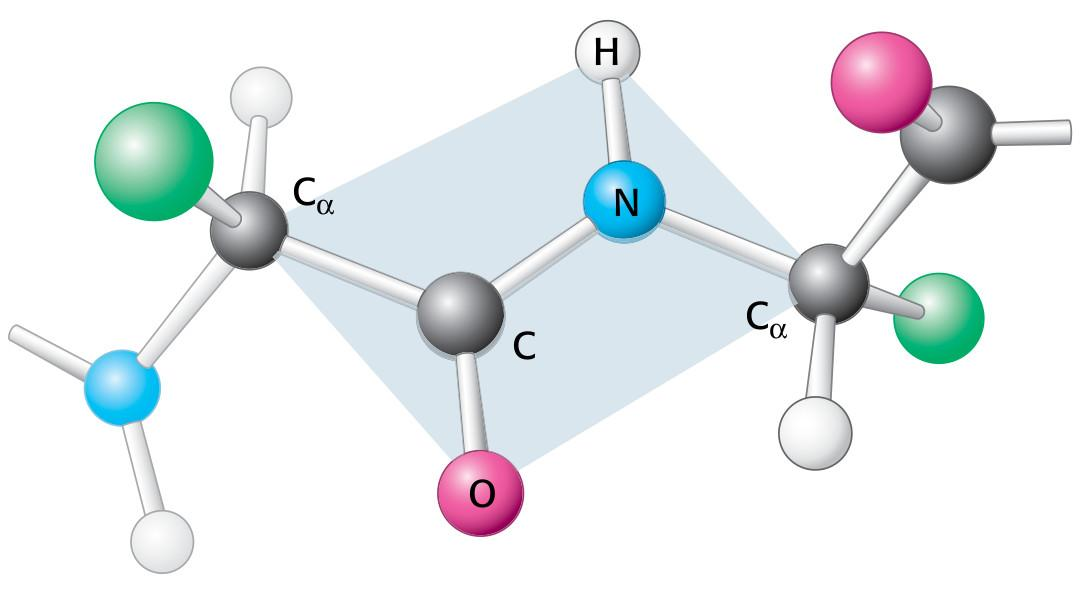
\includegraphics[width=\linewidth]{./literature_review/proteins/secundary_structure/img/trans_planar.jpg}
		\caption{\textbf{Planarity of peptide bond, trans}}
		\label{fig:trans}
	~\end{subfigure}
	\caption{
		\textbf{Peptide bond and torsion angles.}
	Green:R-group,
	Black:Carbon,
	Purple:Oxygen, 
	Blue:Nitrogen,
	White:Hydrogen
		\textbf{a.}
	The partial double bond-character character of peptide bonds ensures that 6 atoms lie in the same plane for every pair of amino acids. 
	The peptide bond is shown in trans configuration.
		\textbf{b.}
	In cis configuration, sidechains will experience energetically unfavorable steric clashes.
		\textbf{c.}
	Torsion angles.
	(From \cite{berg2015}).
	}
~\end{figure}
